\documentclass[journal=jacsat,manuscript=suppinfo]{achemso}
\usepackage[utf8]{inputenc}
\usepackage{amsmath,amssymb}
\usepackage{graphicx}
\usepackage{booktabs}
\usepackage{hyperref}

\title{Supporting Information: Mechanistic High-Throughput Screening of HER, OER, and CO$_2$RR in Metal--Organic Frameworks via Equivariant Machine Learning Interatomic Potentials}

\author{Luiz Antonio Ribeiro Junior}
\affiliation{Institute of Physics, University of Bras\'{i}lia (UnB), 70910-900 Bras\'{i}lia, DF, Brazil}
\alsoaffiliation{Department of Physics, Norwegian University of Science and Technology (NTNU), Trondheim, Norway}
\email{ribeirojr.fis@gmail.com}

\begin{document}

\maketitle

\tableofcontents
\newpage

\section{Computational Details and Methodological Protocol}

\subsection{Quantum MOF (QMOF) Ingestion and Electrocatalytic Screening}
The structural dataset was retrieved from the Materials Project MOF Explorer / QMOF database (\cite{qmof2021}), encompassing $>20,000$ DFT-relaxed metal--organic frameworks. To focus on electrocatalytically tractable and experimentally realizable systems, hierarchical filtering was applied:
\begin{enumerate}
    \item \textbf{Experimental Synthesizability:} Only frameworks with validated experimental synthesis records were retained ($\mathrm{synthesized} = \mathrm{True}$).
    \item \textbf{Active Transition Metal Nodes:} Filtered for redox-active $3d$, $4d$, and $5d$ transition metals ($\mathrm{Co, Cu, Fe, Mn, Mo, Ni, Ru, Zn, Zr}$).
    \item \textbf{Pore Accessibility:} Retained systems with Pore Limiting Diameter ($\mathrm{PLD} \ge 2.5\,\text{\AA}$) to permit unhindered diffusion of $\mathrm{H_2O}$ ($2.65\,\text{\AA}$) and $\mathrm{CO_2}$ ($3.30\,\text{\AA}$).
    \item \textbf{Unit Cell Atom Count:} $N_{\mathrm{atoms}} \le 200$ to maintain structural tractability for precision equivariant MLIP relaxation and localized vibrational thermochemistry.
\end{enumerate}

\subsection{Automated Open Metal Site (OMS) and Coordination Vector Algorithm}
For each framework, the coordination sphere around the transition metal nodes was evaluated within a radial cutoff $R = 2.5\,\text{\AA}$. The outward open coordination unit vector $\hat{u}_{\mathrm{open}}$ pointing toward the pore channel was computed as:
\begin{equation}
    \vec{v}_{\mathrm{open}} = -\sum_{i=1}^{\mathrm{CN}} \frac{\vec{r}_{\mathrm{ligand},i} - \vec{r}_{\mathrm{metal}}}{\|\vec{r}_{\mathrm{ligand},i} - \vec{r}_{\mathrm{metal}}\|}, \quad \hat{u}_{\mathrm{open}} = \frac{\vec{v}_{\mathrm{open}}}{\|\vec{v}_{\mathrm{open}}\|}
\end{equation}
Seven reaction intermediates were attached along $\hat{u}_{\mathrm{open}}$:
\begin{itemize}
    \item \textbf{HER:} $*H$ ($d_{\mathrm{M-H}} = 1.55\,\text{\AA}$).
    \item \textbf{OER:} $*OH$ ($1.85\,\text{\AA}$), $*O$ ($1.68\,\text{\AA}$), $*OOH$ ($1.85\,\text{\AA}$, $\angle\mathrm{MOO} = 110^\circ$).
    \item \textbf{CO$_2$RR:} $*COOH$ ($1.95\,\text{\AA}$, C-bound), $*CO$ ($1.85\,\text{\AA}$, C-bound), $*OCHO$ ($1.95\,\text{\AA}$, O-bound).
\end{itemize}

\subsection{Two-Tier MLIP Strategy: CHGNet and MACE-MP-0}
Calculations were orchestrated via the Atomic Simulation Environment (ASE) with CUDA acceleration:
\begin{enumerate}
    \item \textbf{Tier 1 (CHGNet):} Rapid pre-relaxation ($f_{\mathrm{max}} < 0.10\,\text{eV/\AA}$, BFGS) to relieve initial steric contacts and verify framework stability.
    \item \textbf{Tier 2 (MACE-MP-0):} Higher-order equivariant message passing relaxation in double precision ($\mathrm{float64}$, $f_{\mathrm{max}} < 0.03\,\text{eV/\AA}$) to determine ground-state electronic energies $E_{\mathrm{MLIP}}$.
    \item \textbf{Epistemic Uncertainty Filter:} $\sigma_{\mathrm{MLIP}} = |E_{\mathrm{MACE}} - E_{\mathrm{CHGNet}}| / N_{\mathrm{atoms}}$ to identify sterically congested pore pockets.
\end{enumerate}

\subsection{Partial Hessian Vibrational Analysis (PHVA) and CHE Energetics}
Zero-point vibrational energy (ZPE) and vibrational entropy ($S_{\mathrm{vib}}$) at $T = 298.15\,\mathrm{K}$ were evaluated via finite-difference displacements restricted to the adsorbate atoms. Free energies were calculated within the N{\o}rskov Computational Hydrogen Electrode (CHE) framework:
\begin{equation}
    \Delta G = \Delta E_{\mathrm{MLIP}} + \Delta \mathrm{ZPE} - T \Delta S_{\mathrm{vib}} - eU + k_B T \ln(10) \cdot \mathrm{pH}
\end{equation}
Theoretical overpotentials:
\begin{itemize}
    \item $\eta^{\mathrm{HER}} = |\Delta G_{*H}| / e$
    \item $\eta^{\mathrm{OER}} = \max(\Delta G_1, \Delta G_2, \Delta G_3, \Delta G_4)/e - 1.23\,\mathrm{V}$
    \item $\eta^{\mathrm{CO2RR}} = \max(\Delta G_{*COOH}, \Delta G_{*CO} - \Delta G_{*COOH})/e - (-0.11\,\mathrm{V})$
    \item $\Delta G_{\mathrm{sel}} = \Delta G_{*COOH} - \Delta G_{*H}$
\end{itemize}


\newpage
\section{Supplementary Figures}

\begin{figure}[htbp]
    \centering
    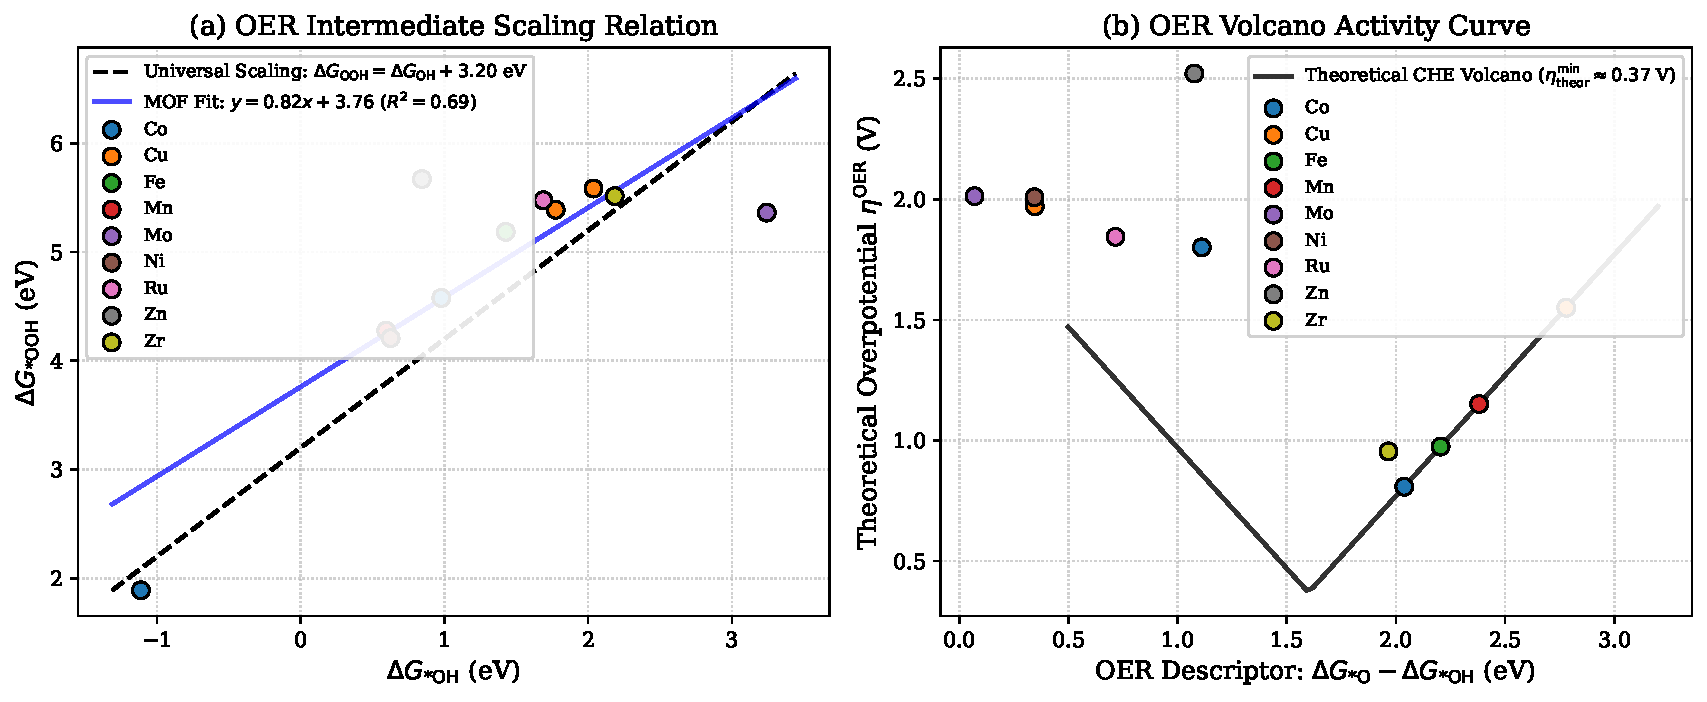
\includegraphics[width=0.95\textwidth]{../figures/fig1_oer_scaling_and_volcano.pdf}
    \caption{\textbf{OER Energetics on MOF Open Metal Sites.} (a) Linear scaling relation between $\Delta G_{*\mathrm{OOH}}$ and $\Delta G_{*\mathrm{OH}}$, benchmarking against the universal oxide scaling line. (b) Theoretical OER activity volcano curve showing overpotential $\eta^{\mathrm{OER}}$ as a function of the descriptor $\Delta G_{*\mathrm{O}} - \Delta G_{*\mathrm{OH}}$.}
    \label{fig:oer_volcano}
\end{figure}

\begin{figure}[htbp]
    \centering
    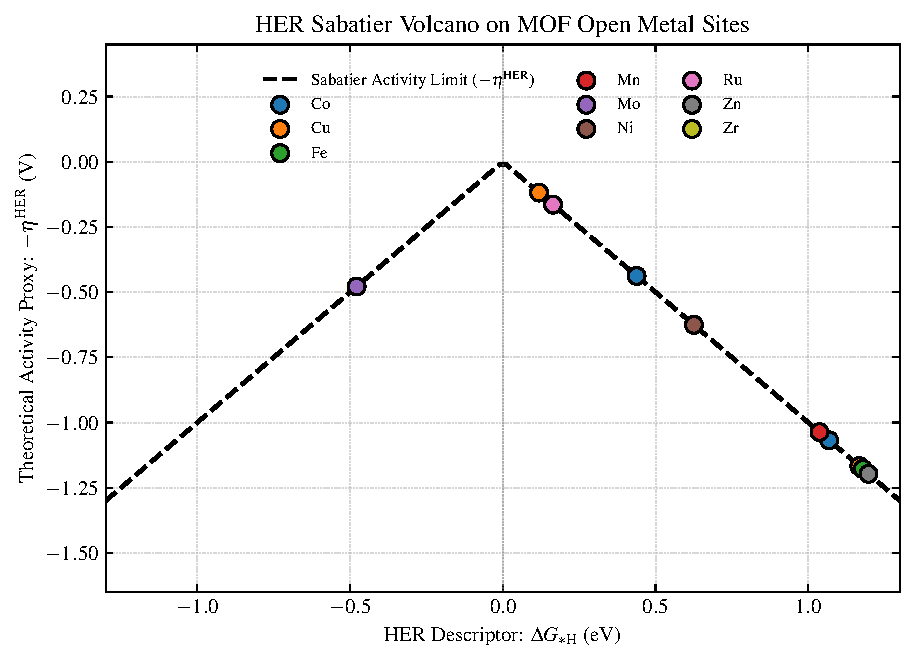
\includegraphics[width=0.65\textwidth]{../figures/fig2_her_volcano.pdf}
    \caption{\textbf{HER Sabatier Volcano Curve.} Theoretical overpotential proxy $-\eta^{\mathrm{HER}}$ as a function of the hydrogen adsorption free energy $\Delta G_{*\mathrm{H}}$. Symmetrical optimal activity peak at $\Delta G_{*\mathrm{H}} = 0\,\mathrm{eV}$.}
    \label{fig:her_volcano}
\end{figure}

\begin{figure}[htbp]
    \centering
    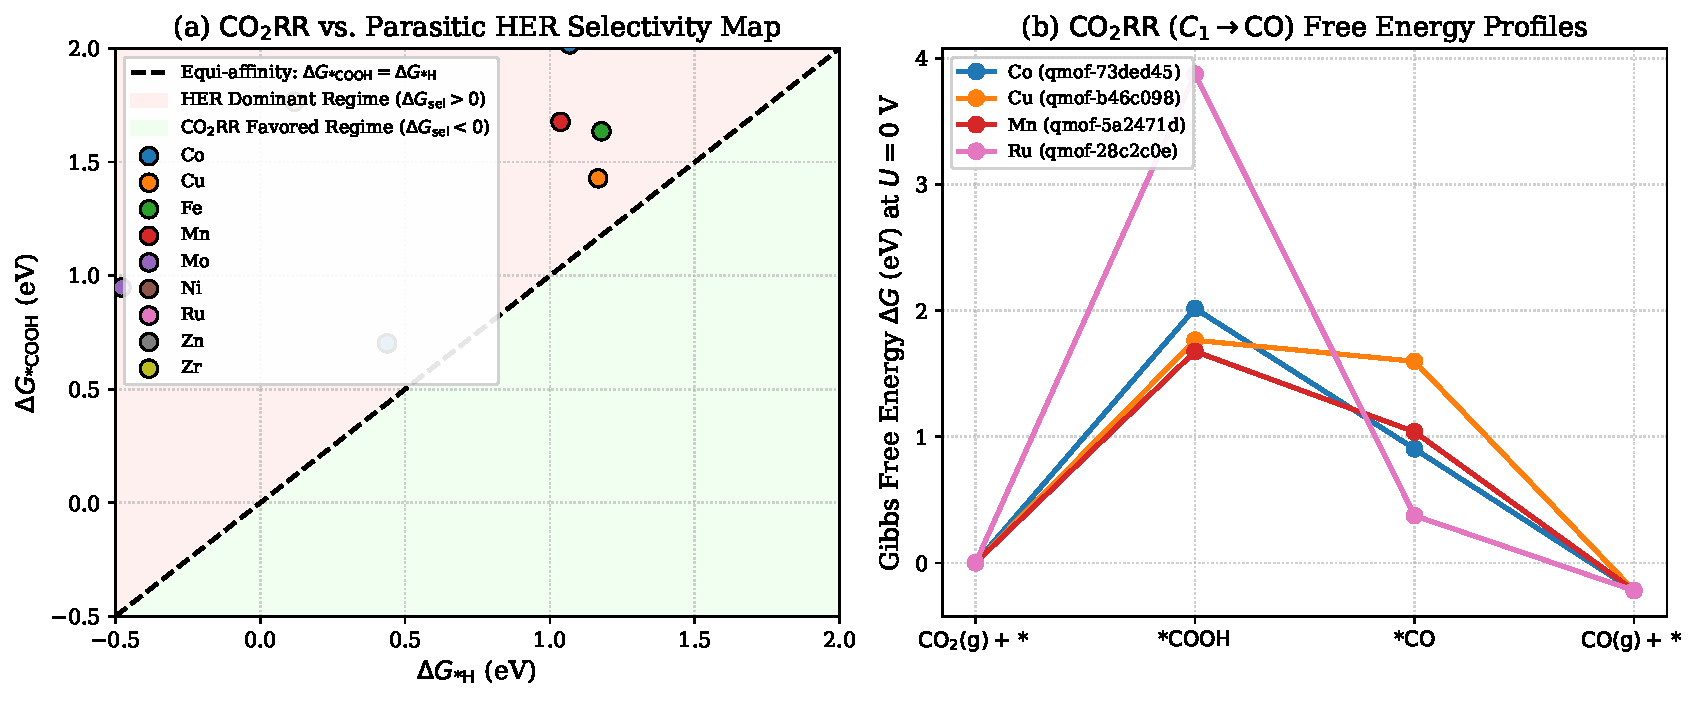
\includegraphics[width=0.95\textwidth]{../figures/fig3_co2rr_her_selectivity.pdf}
    \caption{\textbf{CO$_2$RR vs. HER Selectivity and Reaction Coordinates.} (a) Two-dimensional selectivity map comparing $\Delta G_{*\mathrm{COOH}}$ and $\Delta G_{*\mathrm{H}}$, identifying the boundary between HER-dominant and CO$_2$RR-selective regimes. (b) Free energy profiles for the $C_1 \rightarrow \mathrm{CO}$ reduction pathway across representative MOF metal centers at $U = 0\,\mathrm{V}$.}
    \label{fig:co2rr_selectivity}
\end{figure}

\newpage
\section{Supplementary Tables}
% Electrocatalytic Performance Metrics across MOF Cohort
\begin{tabular}{lllrrrlrr}
\toprule
QMOF ID & Metal & Formula & PLD (\AA) & $\eta^{\mathrm{HER}}$ (V) & $\eta^{\mathrm{OER}}$ (V) & PDS (OER) & $\eta^{\mathrm{CO2RR}}$ (V) & $\Delta G_{\mathrm{sel}}$ (eV) \\
\midrule
qmof-73ded45 & Co & Co6C24H6O18 & 10.99 & 1.07 & 0.81 & *OH -> *O & 1.91 & 0.95 \\
qmof-dc7e5a3 & Co & Co6C24H12O18 & 10.09 & 0.44 & 1.80 & *OOH -> O2 & 0.59 & 0.26 \\
qmof-571d405 & Cu & Cu6C96H36N12O24 & 14.15 & 1.17 & 1.55 & *OH -> *O & 1.32 & 0.26 \\
qmof-b46c098 & Cu & Cu6C24H6O18 & 10.74 & 0.12 & 1.97 & *O -> *OOH & 1.66 & 1.65 \\
qmof-197ad3f & Fe & Fe6C36Cl6H12N18O6 & 18.49 & 1.18 & 0.97 & *OH -> *O & 1.52 & 0.46 \\
qmof-5a2471d & Mn & Mn6C36H12O18 & 11.79 & 1.04 & 1.15 & *OH -> *O & 1.57 & 0.64 \\
qmof-dd825f1 & Mo & Mo4C68H72N16O16 & 4.85 & 0.48 & 2.01 & * -> *OH & 0.84 & 1.43 \\
qmof-02e961c & Ni & Ni3C78H48N12O12 & 35.34 & 0.63 & 2.01 & *O -> *OOH & 15.17 & 14.65 \\
qmof-28c2c0e & Ru & Ru2C38F16H12N4O10 & 5.32 & 0.16 & 1.84 & *O -> *OOH & 3.77 & 3.71 \\
qmof-8deddd1 & Zn & Zn6C42H18O18 & 16.27 & 1.20 & 2.52 & *O -> *OOH & 2.71 & 1.62 \\
qmof-9bfdab6 & Zr & Zr6C80H60O32 & 6.87 & 2.22 & 0.96 & * -> *OH & 1.57 & -0.54 \\
\bottomrule
\end{tabular}


\end{document}
